\externaldocument{../appendix/chapter_app}
\externaldocument{../4/chapter_algorithm}
\externaldocument{../3/chapter_modeling}
\startchapter{Proof of Concept}
\label{chapter:Exp}
In this section, I present two experiments I did for the proof of concept of the communication analysis though execution traces.

These experiments aimed to test the model for communication analysis and the identification algorithms. By these experiment, it should be able to know if the captured dual\_traces contain sufficient information of the communication model in Chapter\ref{chapter:Mod}. They also verify the design of the some algorithms, for their correctness.  

User case study is not included in this thesis and can be the future work. The feature prototype implementation is not evaluated and can be part of the user case study. But I used the implemented feature on Atlantis to conduct the experiments.

I first present the design of the experiments and their result. And then, I discuss the result of the experiments.  

\section{Experiments}
In this section, I describe the design of the evaluation. Two Evaluation experiments are conducted for this evaluation. All the programs in these two experiments were written in C++ and the source code can be found in Section\ref{expcode}. Our search partner DRDC provided the captured traces, the used .dll files and  the source code of the programs for the experiments.

Evaluation results are provided for each experiment. Both of the conducted experiments are about named pipe communication method. The following two subsections provides the details of the experiments and their result.

\subsection{Experiment 1}
In the first experiment, two programs communicated with each other through a synchronous Named pipe channel. One of the programs acted as the Named pipe server while the other as the client. Figure\ref{exp1} is the sequence diagram of the interaction between the server and client. Traces were captured while these two program were running and interacting. The two captured traces are analysis as dual\_trace $exp1$ in this experiment. I used the implemented features in Atlantis to analyse this dual\_trace. I ran the ``Stream identification" and ``Communication identification" operations for this dual\_trace. The identified streams, communication and the processing time are listed in Figure\ref{result1}.

\begin{figure}[H]
\centerline{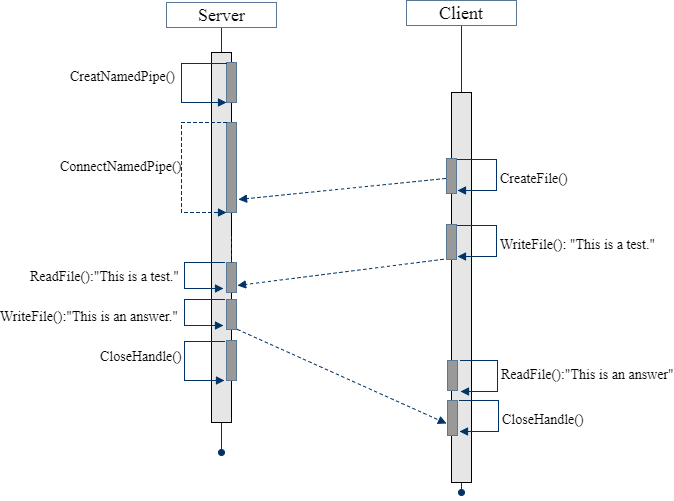
\includegraphics[scale=0.7]{Figures/exp1}}
 \caption{Sequence Diagram of Experiment 1}
\label{exp1}
\end{figure}

\begin{figure}[H]
\centerline{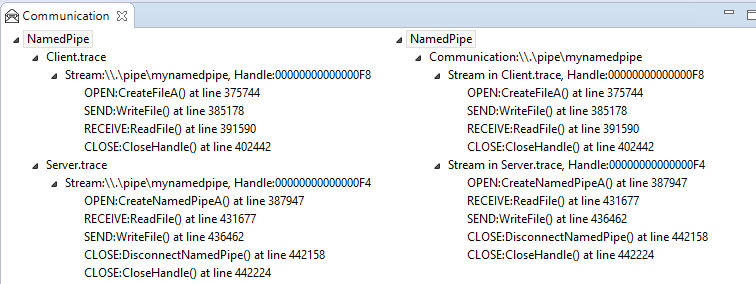
\includegraphics[scale=0.6]{Figures/result1}}
 \caption{Identification result of $exp1$}
\label{result1}
\end{figure}

\subsection{Experiment 2}
In the second experiment, one program was running as the Named pipe server. In this server program, four named pipes were created and can be connected by up to four client at a time. Two other programs as the Named pipe clients connected to this server. Those two clients (client 1 and client 2) used the identical program but run in sequence. Figure\ref{exp2} is the sequence diagram of  the interaction among the server and clients. The function calls' sequence is only a possible combination from analyzing the source code. The real happening sequence can be vary from program run to program run. Traces were captured at the time when these five programs were running and interacting. One trace for each program. I only analyzed  three traces which are considered as two dual\_traces, $exp2.1$ and $exp2.2$. $exp2.1$ consist of traces of server and client 1 and $exp2.2$ consist of traces of server and client 2. I also ran the ``Stream identification" and ``Communication identification" operations for these two dual\_trace. The identified streams, communication and the processing time are listed in Figure\ref{result21} and Figure\ref{result22}.

\begin{figure}[H]
\centerline{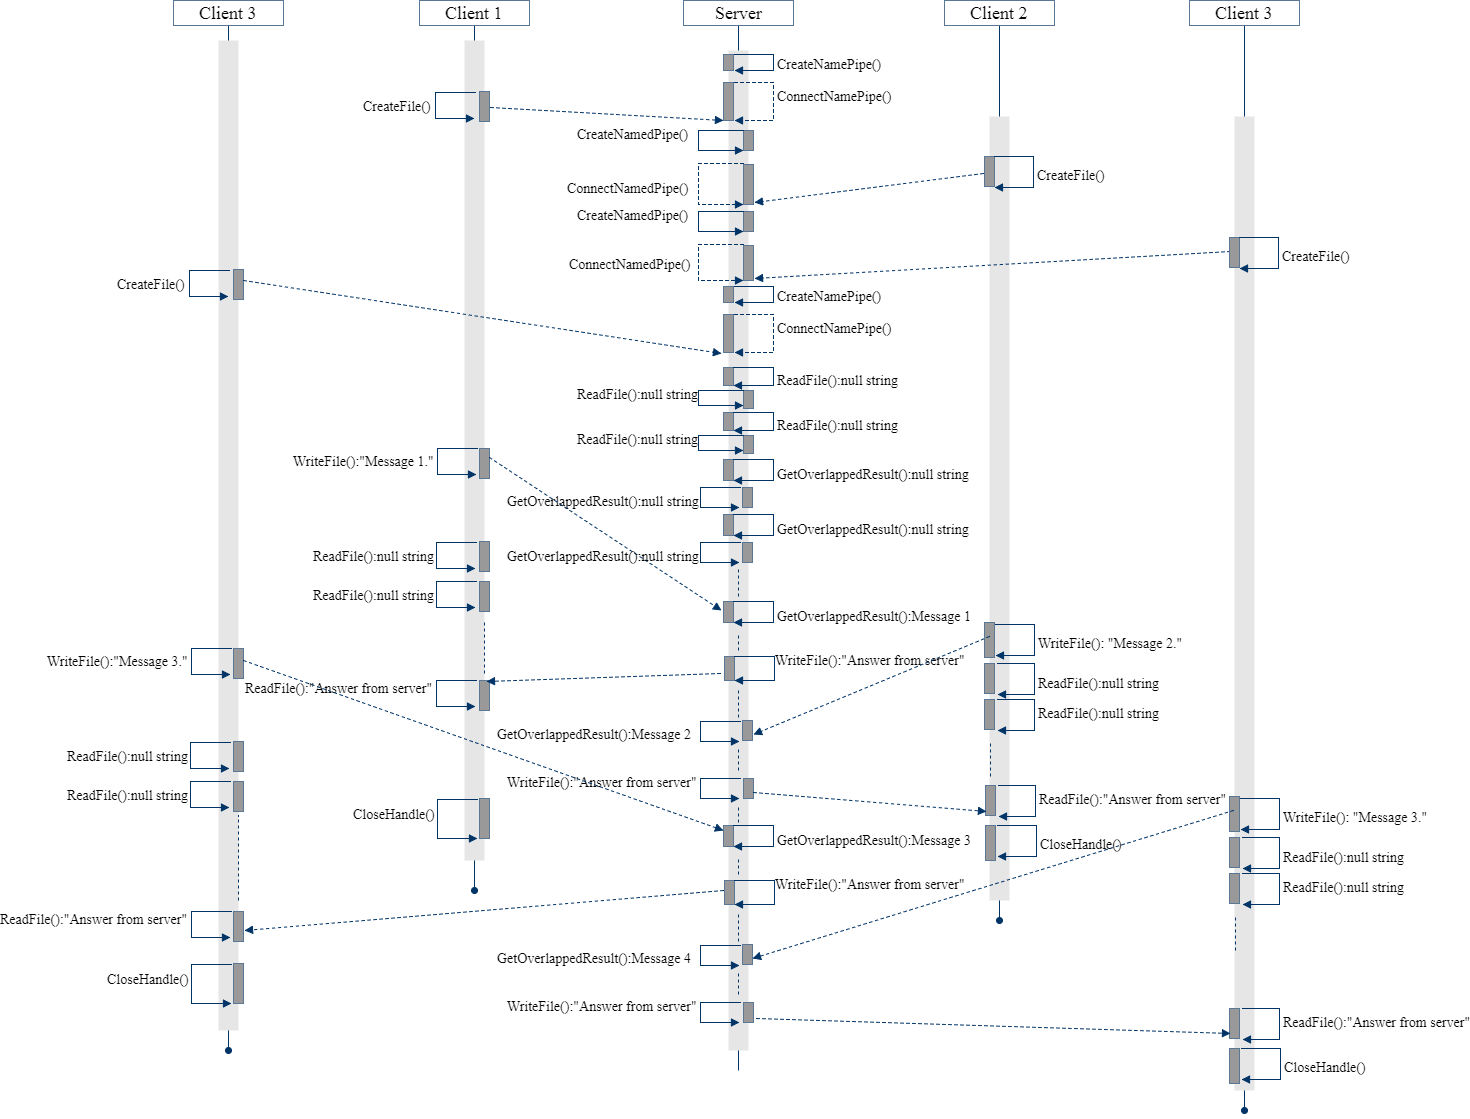
\includegraphics[scale=0.48]{Figures/exp2}}
 \caption{Sequence Diagram of Experiment 2}
\label{exp2}
\end{figure}

\begin{figure}[H]
\centerline{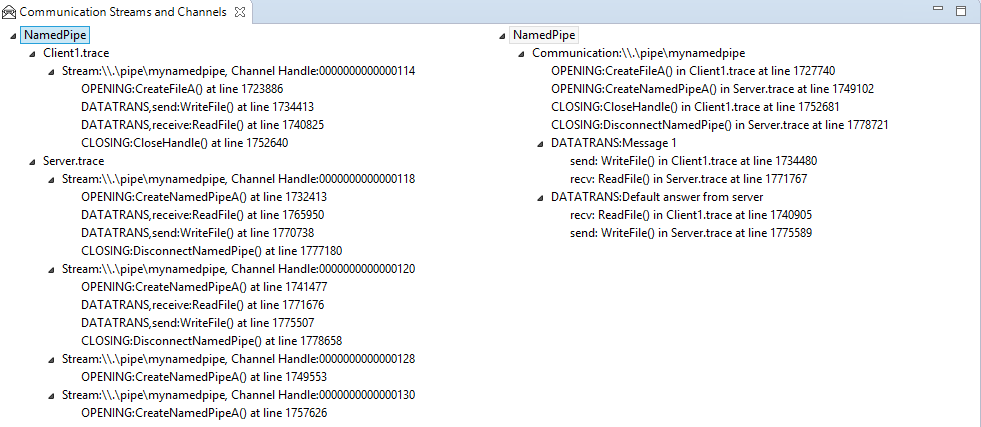
\includegraphics[scale=0.6]{Figures/result21}}
 \caption{Identification result of $exp2.1$}
\label{result21}
\end{figure}

\begin{figure}[H]
\centerline{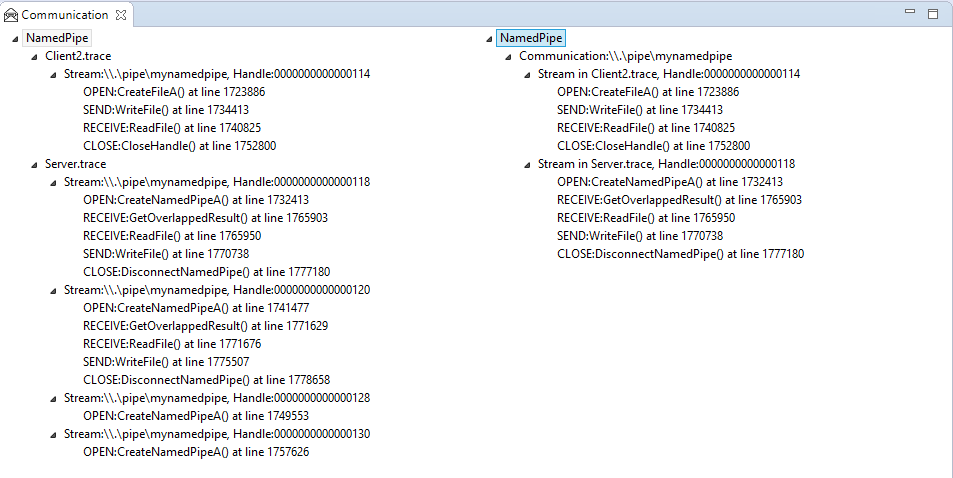
\includegraphics[scale=0.6]{Figures/result22}}
 \caption{Identification result of $exp2.1$}
\label{result22}
\end{figure}


\section{Discussion}
In the result of $exp1$, there are one stream identified in client trace and one in server trace, and these two streams are matched into a communication of this dual\_trace. This identification result represents the actual communication happen between the named pipe server and client.
In the result of $exp2.1$ and $exp2.2$, there are one stream identified in client traces and four in server trace respectively for each dual\_trace. The streams are further matched and verified and eventually one communication is identified for each dual\_trace. The result aligns to the sequence diagram in Figure\ref{exp2}.


   




